\subsubsection{UC\theuccount-PR - Producer Redmine invia messaggio al Gestore Personale}
    \begin{figure}[H]
		\centering
		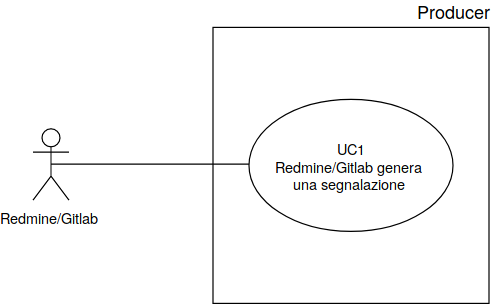
\includegraphics[width=0.7\textwidth]{img/UC1.png}\\
		\caption{UC\theuccount-PR - Producer Redmine invia messaggio al Gestore Personale}
	\end{figure}
	\begin{itemize}
		\item \textbf{Codice}: UC\theuccount-PR.
		\item \textbf{Titolo}: Producer Redmine invia messaggio al Gestore Personale.
		\item \textbf{Attori primari}: Producer Redmine.
		\item \textbf{Descrizione}:
		 il sistema qui è Gestore Personale ed è interno al sistema
		 Butterfly. Il Producer Redmine, dopo aver ricevuto una
		 segnalazione da Redmine, elabora il messaggio e lo invia al Gestore Personale.
		 Il messaggio finale, una volta terminata l'elaborazione, conterrà i campi:
		 \begin{itemize}
		 	\item Project
		 	\item Topic
		 	\item Subject e opzionalmente:
		 	\begin{itemize}
		 		\item Description
		 	\end{itemize}
		 \end{itemize}
		\item \textbf{Precondizione}: il Producer Redmine ha ricevuto una segnalazione da Redmine.
		\item \textbf{Postcondizione}: il Producer Redmine ha elaborato e inviato al Gestore Personale il messaggio.
		\item \textbf{Scenario principale}: 
		\begin{enumerate}
			\item Producer Redmine procede all'invio del messaggio al gestore personale.
		\end{enumerate}
		
	\end{itemize}

	\paragraph{UC\theuccount.1-PR - Producer Redmine invia messaggio di apertura issue al Gestore Personale}
	\begin{figure}[H]
		\centering
		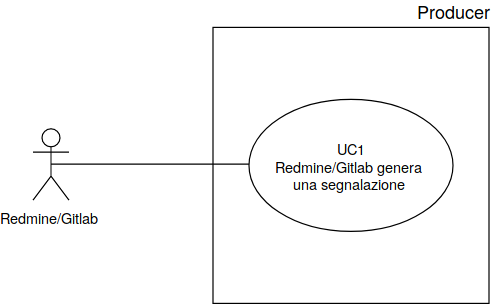
\includegraphics[width=0.7\textwidth]{img/UC1.png}\\
		\caption{UC\theuccount.1-PR - Producer Redmine invia messaggio di apertura issue al Gestore Personale}
	\end{figure}
	\begin{itemize}
		\item \textbf{Codice}: UC\theuccount.1-PR.
		\item \textbf{Titolo}: Producer Redmine invia messaggio di apertura issue al Gestore Personale.
		\item \textbf{Attori primari}: Producer Redmine.
		\item \textbf{Descrizione}:il sistema qui è il Gestore Personale
		ed è interno al sistema Butterfly. Il Producer Redmine, dopo aver
		ricevuto una segnalazione di apertura issue da Redmine, elabora
		il messaggio e lo invia al Gestore Personale.
		Il messaggio finale, una volta terminata l'elaborazione, conterrà i campi:
		\begin{itemize}
			\item Project
			\item Topic
			\item Subject e opzionalmente:
			\begin{itemize}
				\item Description
			\end{itemize}
		\end{itemize}
		\item \textbf{Precondizione}: il Producer Redmine ha ricevuto una segnalazione da Redmine.
		\item \textbf{Postcondizione}: il Producer Redmine ha elaborato e inviato al Gestore Personale il messaggio di apertura issue.
		\item \textbf{Scenario principale}: 
		\begin{enumerate}
			\item Producer Redmine procede all'invio del messaggio di
			apertura issue al gestore personale.
		\end{enumerate}
		
	\end{itemize}

	\paragraph{UC\theuccount.2-PR - Producer Redmine invia messaggio di modifica issue al Gestore Personale}
	\begin{figure}[H]
		\centering
		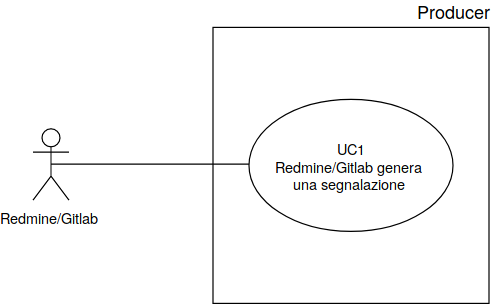
\includegraphics[width=0.7\textwidth]{img/UC1.png}\\
		\caption{UC\theuccount.2-PR - Producer Redmine invia messaggio di modifica issue al Gestore Personale}
	\end{figure}
	\begin{itemize}
		\item \textbf{Codice}: UC\theuccount.2-PR.
		\item \textbf{Titolo}: Producer Redmine invia messaggio di modifica issue al Gestore Personale
		\item \textbf{Attori primari}: Producer Redmine.
		\item \textbf{Descrizione}:il sistema qui è il Gestore Personale
		ed è interno al sistema Butterfly. Il Producer Redmine, dopo aver
		ricevuto una segnalazione di modifica issue da Redmine, elabora
		il messaggio e lo invia al Gestore Personale.
		Il messaggio finale, una volta terminata l'elaborazione, conterrà i campi:
		\begin{itemize}
			\item Project
			\item Topic
			\item Subject e opzionalmente:
			\begin{itemize}
				\item Description
			\end{itemize}
		\end{itemize}
		\item \textbf{Precondizione}: il Producer Redmine ha ricevuto una segnalazione da Redmine.
		\item \textbf{Postcondizione}: il Producer Redmine ha elaborato e inviato al Gestore Personale il messaggio di modifica issue.
		\item \textbf{Scenario principale}: 
		\begin{enumerate}
			\item Producer Redmine procede all'invio del messaggio di
			modifica issue al gestore personale.
		\end{enumerate}
		
	\end{itemize}